\chapter{Sprint 5 : Pipeline DevOps et Gestion GitOps}
\section{Introduction}
Le Sprint 5 marque une étape clé dans l’évolution de notre plateforme en introduisant un pipeline DevOps robuste basé sur GitHub Actions et une démarche GitOps avec ArgoCD. Fort des avancées des sprints précédents, ce sprint se concentre sur l’automatisation des processus de construction, de test et de déploiement via des workflows GitHub Actions, permettant la création et la mise à jour d’images Docker de manière fluide et intégrée avec DockerHub et SonarQube pour assurer la qualité du code. Parallèlement, l’adoption d’une approche GitOps avec ArgoCD, synchronisée avec le dépôt \texttt{k8s-manifests}, garantit une gestion centralisée et automatisée des déploiements sur MicroK8s, avec des capacités de surveillance et de rollback pour une fiabilité accrue. Ces améliorations visent à optimiser l’efficacité opérationnelle, renforcer la sécurité via une gestion des secrets Kubernetes, et poser les bases d’une infrastructure évolutive et maintenable.
\section{Backlog du Sprint 5}
Le tableau 7.1 représente le backlog du cinquième sprint. Ce tableau détaille les cas d’utilisation, leurs priorités et tâches associées.
\newpage
\begin{table}[!ht]
      \begin{adjustwidth}{-3.5cm}{-3.5cm}
      \vspace{-1cm}
      \centering
      \caption{Backlog du Sprint 5 : Pipeline DevOps et Gestion GitOps}
      \begin{tabular}{|p{5cm}|p{2cm}|p{8cm}|}
      \hline
      \cellcolor[rgb]{0.832,0.832,0.832}Cas d’utilisation & \cellcolor[rgb]{0.832,0.832,0.832}Priorité & \cellcolor[rgb]{0.832,0.832,0.832}Tâche \\
      \hline
      Installation Automatisée & 4 & Créer un playbook Ansible pour installer MicroK8s, ArgoCD et leurs dépendances, incluant les add-ons Ingress et DNS, pour un déploiement rapide et fiable et configurer ArgoCD pour synchroniser automatiquement avec le dépôt k8s-manifests et gérer les déploiements \\
      \hline
      Workflows CI & 5 & Implémenter des workflows GitHub Actions pour construire et pousser les images Docker vers DockerHub, avec mise à jour des tags dans k8s-manifests. \\
      \hline
      Runner SonarQube & 5 & Configurer un runner auto-hébergé pour exécuter SonarScanner et analyser la qualité du code dans l’instance SonarQube locale. \\
      \hline
      Gestion des Secrets & 5 & Encoder les variables sensibles (identifiants DB, tokens API) en Base64 et les gérer via des secrets Kubernetes. \\
      \hline
      Exposition des Services & 6 & Déployer des règles Ingress pour exposer les services frontend, backend et SonarQube. \\
      \hline
      Surveillance et Rollback & 6 & Vérifier la surveillance automatique des déploiements et le rollback natif d’ArgoCD en cas d’échec d’un nouveau pod. \\
      \hline
      \end{tabular}
      \end{adjustwidth}
\end{table}

\section{Raffinement des cas d’utilisation}
Dans cette section, les cas d'utilisation du Sprint 5 sont raffinés avec des acteurs, des pré-conditions, des post-conditions, des scénarios de base et des exceptions pour assurer une compréhension claire et une exécution efficace.
\subsection{Identification des acteurs du Sprint 5}
Les acteurs de ce sprint sont : \\
    \textbf{Ingénieur DevOps} : Responsable de l’installation et de la configuration automatisée de MicroK8s et ArgoCD, de la configuration du runner auto-hébergé pour SonarQube, de la gestion des secrets Kubernetes, de l’exposition des services via Ingress, et de la validation de la surveillance et du rollback avec ArgoCD. \\
    \textbf{Développeur} : Impliqué dans la mise en œuvre et l’exécution des workflows CI avec GitHub Actions pour construire et déployer les images Docker, ainsi que dans la mise à jour des manifests dans le dépôt k8s-manifests. \\
\subsection{Raffinement du cas d'utilisation <<Installation Automatisée>>}
Le cas d’utilisation « Installation Automatisée » vise à poser les fondations de l’infrastructure du projet en automatisant l’installation et la configuration de MicroK8s et ArgoCD. Cette étape est cruciale pour garantir un déploiement rapide et fiable du cluster Kubernetes, ainsi qu’une gestion automatisée des déploiements via une synchronisation continue avec le dépôt k8s-manifests.
\begin{table}[!ht]
      \centering
      \caption{Description textuelle du Cas d’utilisation «Installation Automatisée»}
      \label{tab:installation_automatisee}
      \renewcommand{\arraystretch}{1.2}
      \begin{tabular}{|p{4.2cm}|p{11cm}|}
      \hline
      \textbf{Cas d'utilisation} & Installation Automatisée \\
      \hline
      \textbf{Acteur} & Ingénieur DevOps \\
      \hline
      \textbf{Pré-conditions} & Environnement cible accessible (serveur ou machine locale). \newline Outils Ansible et dépendances installés sur la machine. \newline Accès réseau aux dépôts pour MicroK8s et ArgoCD. \\
      \hline
      \textbf{Post-conditions} & MicroK8s, ArgoCD, et add-ons (Ingress, DNS) sont installés et fonctionnels. \newline ArgoCD est configuré pour synchroniser avec le dépôt k8s-manifests. \\
      \hline
      \textbf{Scénario de Base} & 
      1. L’ingénieur DevOps exécute le playbook Ansible. \newline
      2. Ansible installe MicroK8s, ArgoCD, et configure les add-ons (Ingress, DNS). \newline
      3. ArgoCD est configuré pour se connecter au dépôt k8s-manifests. \newline
      4. Une application est déployée pour valider la synchronisation automatique. \\
      \hline
      \textbf{Exceptions} & 
      Échec d’installation (connexion réseau interrompue, dépendances manquantes, erreurs Ansible). \newline Problème de synchronisation ArgoCD (dépôt inaccessible ou mal configuré). \\
      \hline
      \end{tabular}
  \end{table}
  \subsection{Raffinement du cas d'utilisation <<Workflows CI>>}
  Le cas d’utilisation « Workflows CI » se concentre sur l’automatisation du processus de construction des applications via GitHub Actions. Cette tâche est essentielle pour permettre aux développeurs de déployer rapidement de nouvelles versions des applications backend et frontend, tout en assurant une intégration fluide avec DockerHub et le dépôt k8s-manifests.
  \newpage
  \begin{table}[!ht]
      \centering
      \caption{Description textuelle du Cas d’utilisation «Workflows CI»}
      \label{tab:workflows_ci}
      \renewcommand{\arraystretch}{1.2}
      \begin{tabular}{|p{4.2cm}|p{11cm}|}
      \hline
      \textbf{Cas d'utilisation} & Workflows CI \\
      \hline
      \textbf{Acteur} & Développeur \\
      \hline
      \textbf{Pré-conditions} & Dépôt GitHub configuré avec un workflow GitHub Actions. \newline Accès à DockerHub avec des identifiants valides. \newline Dépôt k8s-manifests existant. \\
      \hline
      \textbf{Post-conditions} & Les images Docker sont construites et poussées vers DockerHub. \newline Les tags dans k8s-manifests sont mis à jour. \\
      \hline
      \textbf{Scénario de Base} & 
      1. Le développeur pousse du code ou ouvre une pull request sur la branche main. \newline
      2. GitHub Actions déclenche le workflow correspondant (backend ou frontend). \newline
      3. Le workflow construit l’application (Maven pour backend, Node.js pour frontend). \newline
      4. L’image Docker est poussée vers DockerHub avec les tags github.sha et latest. \newline
      5. Le tag dans k8s-manifests est mis à jour et poussé vers GitHub. \\
      \hline
      \textbf{Exceptions} & 
      Échec de construction (dépendances manquantes, erreurs de compilation). \newline Problème d’authentification à DockerHub. \newline Échec de mise à jour de k8s-manifests (conflit Git ou token invalide). \\
      \hline
      \end{tabular}
  \end{table}
  \subsection{Raffinement du cas d'utilisation <<Runner SonarQube>>}
  Le cas d’utilisation « Runner SonarQube » vise à garantir la qualité du code backend en intégrant une analyse automatisée via SonarQube, exécutée sur un runner auto-hébergé. Cette tâche est cruciale pour maintenir des standards élevés de qualité logicielle et identifier les problèmes potentiels avant le déploiement.
  \newpage
  \begin{table}[!ht]
      \centering
      \caption{Description textuelle du Cas d’utilisation «Runner SonarQube»}
      \label{tab:runner_sonarqube}
      \renewcommand{\arraystretch}{1.2}
      \begin{tabular}{|p{4.2cm}|p{11cm}|}
      \hline
      \textbf{Cas d'utilisation} & Runner SonarQube \\
      \hline
      \textbf{Acteur} & Ingénieur DevOps \\
      \hline
      \textbf{Pré-conditions} & Instance SonarQube locale accessible (192.168.2.189). \newline Runner auto-hébergé configuré et connecté à GitHub Actions. \newline Code backend prêt à être analysé. \\
      \hline
      \textbf{Post-conditions} & Le runner exécute SonarScanner avec succès. \newline Les résultats d’analyse sont visibles dans SonarQube local. \\
      \hline
      \textbf{Scénario de Base} & 
      1. L’ingénieur DevOps configure le runner auto-hébergé. \newline
      2. Le workflow GitHub Actions déclenche l’analyse via SonarScanner. \newline
      3. Le runner envoie les résultats à l’instance SonarQube locale. \newline
      4. L’ingénieur vérifie les rapports dans l’interface SonarQube. \\
      \hline
      \textbf{Exceptions} & 
      Échec de connexion au runner (erreur de configuration GitHub). \newline SonarQube inaccessible (problème réseau ou serveur hors ligne). \newline Erreur d’analyse (configuration SonarScanner incorrecte). \\
      \hline
      \end{tabular}
  \end{table}
  \subsection{Raffinement du cas d'utilisation <<Gestion des Secrets>>}
  Le cas d’utilisation « Gestion des Secrets » se concentre sur la sécurisation des données sensibles utilisées par les applications déployées sur Kubernetes. Cette tâche est essentielle pour protéger les identifiants et tokens API, garantissant que seules les applications autorisées y ont accès.
  \begin{table}[!ht]
      \centering
      \caption{Description textuelle du Cas d’utilisation «Gestion des Secrets»}
      \label{tab:gestion_secrets}
      \renewcommand{\arraystretch}{1.2}
      \begin{tabular}{|p{4.2cm}|p{11cm}|}
      \hline
      \textbf{Cas d'utilisation} & Gestion des Secrets \\
      \hline
      \textbf{Acteur} & Ingénieur DevOps \\
      \hline
      \textbf{Pré-conditions} & Cluster Kubernetes (MicroK8s) opérationnel. \newline Variables sensibles (identifiants DB, tokens API) identifiées. \\
      \hline
      \textbf{Post-conditions} & Les secrets sont créés et accessibles aux services backend et frontend. \\
      \hline
      \textbf{Scénario de Base} & 
      1. L’ingénieur DevOps encode les identifiants DB et tokens API en Base64. \newline
      2. L’ingénieur crée des secrets Kubernetes. \newline
      3. Les services backend et frontend intègrent les secrets dans leurs configurations. \newline
      4. L’accès aux ressources est testé avec succès. \\
      \hline
      \textbf{Exceptions} & 
      Erreur d’encodage Base64 ou création de secret (syntaxe incorrecte). \newline Accès refusé aux secrets (configuration Kubernetes incorrecte). \newline Problème de réseau ou d’authentification aux ressources externes. \\
      \hline
      \end{tabular}
  \end{table}
  \newpage
  \subsection{Raffinement du cas d'utilisation <<Exposition des Services>>}
  Le cas d’utilisation « Exposition des Services » permet aux utilisateurs d’accéder aux applications backend, frontend et SonarQube via des URLs publiques. Cette tâche est importante pour rendre les services opérationnels et accessibles, tout en assurant une configuration correcte des règles Ingress.
  \begin{table}[!ht]
      \centering
      \caption{Description textuelle du Cas d’utilisation «Exposition des Services»}
      \label{tab:exposition_services}
      \renewcommand{\arraystretch}{1.2}
      \begin{tabular}{|p{4.2cm}|p{11cm}|}
      \hline
      \textbf{Cas d'utilisation} & Exposition des Services \\
      \hline
      \textbf{Acteur} & Ingénieur DevOps \\
      \hline
      \textbf{Pré-conditions} & Cluster MicroK8s avec Ingress activé. \newline Services backend, frontend et SonarQube déployés. \\
      \hline
      \textbf{Post-conditions} & Les services frontend, backend et SonarQube sont accessibles via des URLs Ingress. \\
      \hline
      \textbf{Scénario de Base} & 
      1. L’ingénieur DevOps configure les règles Ingress pour les services. \newline
      2. Les services sont exposés via des URLs (ex. : frontend.192.168.2.189.nip.io). \newline
      3. L’ingénieur teste l’accès aux services via un navigateur ou cURL. \newline
      4. Les règles sont déboguées si nécessaire. \\
      \hline
      \textbf{Exceptions} & 
      Échec de configuration Ingress (erreur DNS, conflit de règles). \newline Service inaccessible (port bloqué ou pod non healthy). \\
      \hline
      \end{tabular}
  \end{table}
  \subsection{Raffinement du cas d'utilisation <<Surveillance et Rollback>>}
  Le cas d’utilisation « Surveillance et Rollback » vise à valider les capacités natives d’ArgoCD pour surveiller les déploiements et effectuer des rollbacks automatiques en cas d’échec. Cette tâche est essentielle pour garantir la stabilité des déploiements et documenter leur gestion via l’interface ArgoCD.
  \newpage
  \begin{table}[!ht]
      \centering
      \caption{Description textuelle du Cas d’utilisation «Surveillance et Rollback»}
      \label{tab:surveillance_rollback}
      \renewcommand{\arraystretch}{1.2}
      \begin{tabular}{|p{4.2cm}|p{11cm}|}
      \hline
      \textbf{Cas d'utilisation} & Surveillance et Rollback \\
      \hline
      \textbf{Acteur} & Ingénieur DevOps \\
      \hline
      \textbf{Pré-conditions} & ArgoCD configuré et synchronisé avec k8s-manifests. \newline Cluster MicroK8s opérationnel avec services déployés. \\
      \hline
      \textbf{Post-conditions} & La surveillance automatique est validée, et un rollback est effectué si un pod échoue. \newline Une capture d’écran de l’UI ArgoCD est disponible. \\
      \hline
      \textbf{Scénario de Base} & 
      1. L’ingénieur DevOps introduit un nouveau pod via une mise à jour dans k8s-manifests. \newline
      2. ArgoCD surveille l’état du pod et attend qu’il soit healthy. \newline
      3. Si le pod échoue, ArgoCD effectue un rollback vers l’état précédent. \\
      \hline
      \textbf{Exceptions} & 
      Échec de détection par ArgoCD (configuration incorrecte). \newline Rollback inefficace (manifests corrompus ou conflit). \\
      \hline
      \end{tabular}
  \end{table}
  \section{Conception}
\subsection{Diagramme de déploiement}
Le diagramme de déploiement illustre le processus d’automatisation et de gestion des déploiements pour le projet, en suivant une approche DevOps et GitOps. Initialement, un développeur pousse le code dans les dépôts GitHub (backend en Java/Maven et frontend en Node.js), déclenchant les workflows CI/CD. Le runner GitHub Actions (cloud) pour le frontend construit et pousse l’image Docker vers Docker Hub, tandis que le runner auto-hébergé pour le backend effectue des tests, analyse le code avec SonarQube local, construit l’image Docker, et met à jour les tags dans le dépôt k8s-manifests. ArgoCD, déployé sur le cluster MicroK8s, détecte les changements dans k8s-manifests et déploie automatiquement les applications backend, frontend, et MySQL, en s’appuyant sur les manifests. Enfin, Ingress expose ces services aux utilisateurs via des routes définies, assurant une accessibilité externe tout en maintenant une synchronisation continue et une surveillance efficace des déploiements.
\newpage
\begin{figure}[h]
      \centering
      \fbox{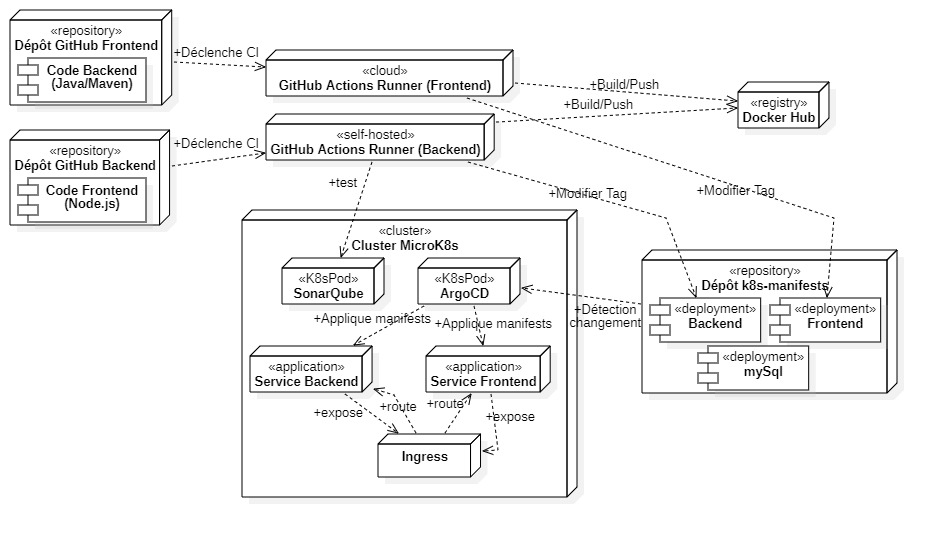
\includegraphics[width=17cm]{images/DeploymentDiagram.jpg}}
      \caption{Diagramme de déploiement du système}
      \label{fig:DeploymentDiagram}
  \end{figure}
\subsection{Architecture du système}
Le diagramme présente une architecture hybride combinant des éléments logiques et physiques, débutant par: \\
\textbf{Ansible} qui installe et configure sur une machine virtuelle un \textbf{Cluster MicroK8s}.\\
Ce cluster est structuré en deux namespaces : l’un dédié aux applications, incluant les pods \textbf{Approbation-frontend}, \textbf{Approbation-backend}, \textbf{Approbation-mysql} et \textbf{Approbation-ollama}, qui communiquent entre eux via des \textbf{Services ClusterIP}, et l’autre dédié à \textbf{ArgoCD} qui synchronise les manifests pour déployer et gérer les pods.\\
Les services sont exposés à l’extérieur grâce à \textbf{Ingress}, qui route le trafic vers des URLs spécifiques. Par exemple, \texttt{frontend.192.168.2.189.nip.io} pour le frontend,\\
\texttt{backend.192.168.2.189.nip.io} pour le backend,\\
\texttt{sonarqube.192.168.2.189.nip.io} pour SonarQube et le port \texttt{30339} est exposé pour permettre l'accès a l'interface d'argoCD.\\
Enfin, un utilisateur accède aux interfaces des pods frontend, backend, SonarQube, et à l’interface d’ArgoCD pour surveiller et administrer les déploiements.
\newpage
\begin{figure}[h]
      \begin{adjustwidth}{-3.5cm}{-3.5cm}
      \centering
      \fbox{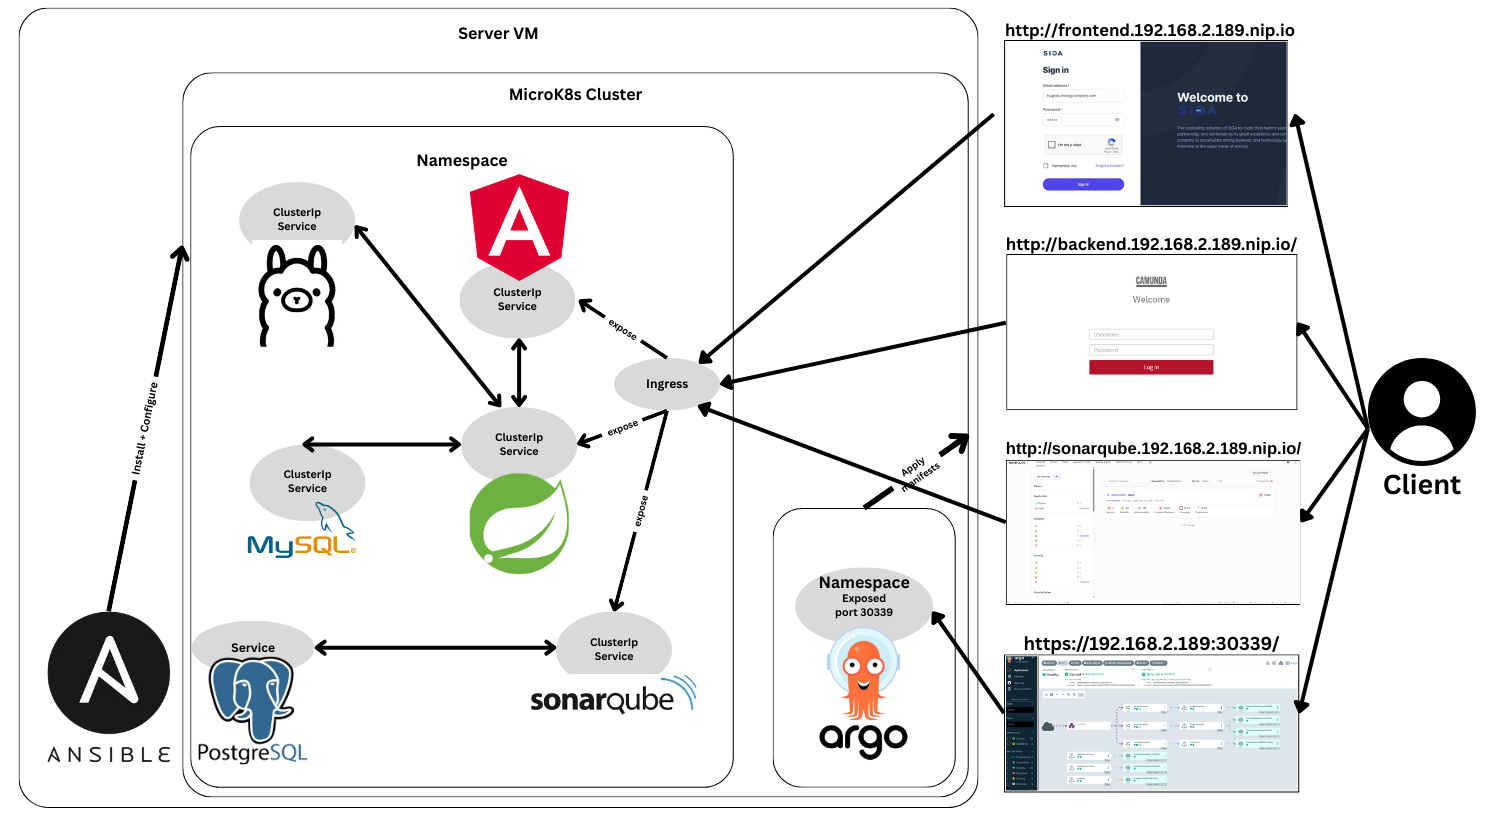
\includegraphics[width=20cm]{images/Server VM (3).png}}
      \caption{Architecture du système}
      \label{fig:sysarch}
      \end{adjustwidth}
  \end{figure}
  \section{Réalisation}
  \subsection{Installation Automatisée}
  \subsubsection{Arborescence des fichiers d'Ansible}
  Cette image montre le contenu du répertoire du projet Ansible, incluant les fichiers \texttt{ansible.cfg}, \texttt{argocd-app-of-apps.yaml}, \texttt{argocd-ns.json}, \texttt{deploy\_argocd\_application.yaml}, \texttt{install\_ansible\_dependencies.yaml}, \texttt{inventory}, \texttt{main.yaml}, \texttt{README.md}, \texttt{setup\_argocd.yaml}, et \texttt{setup\_microk8s.yaml}. Elle illustre l'organisation des fichiers nécessaires pour automatiser l’installation et la gestion du cluster MicroK8s et d’ArgoCD.
  \newpage
  \begin{figure}[h]
      \vspace*{-1cm}
      \begin{adjustwidth}{-3.5cm}{-3.5cm}
      \centering
      \fbox{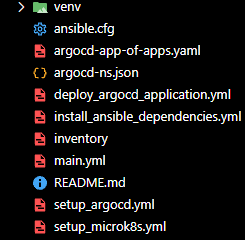
\includegraphics[width=7cm]{images/ansible/1.png}}
      \caption{Répertoire du Projet Ansible}
      \label{fig:ansible00}
      \end{adjustwidth}
  \end{figure}
  \subsubsection{Fichier ansible.cfg}
  Cette image présente le fichier de configuration \texttt{ansible.cfg}, qui spécifie les paramètres par défaut pour Ansible. On y voit les options \texttt{inventory = inventory}, \texttt{host\_key\_checking = False}, \texttt{interpreter\_python = auto\_silent}, et une section \texttt{[privilege\_escalation]} avec \texttt{become = True}, \texttt{become\_method = sudo}, et \texttt{become\_ask\_pass = False} pour gérer les privilèges d’administration.
    \begin{figure}[h]
      \begin{adjustwidth}{-3.5cm}{-3.5cm}
      \centering
      \fbox{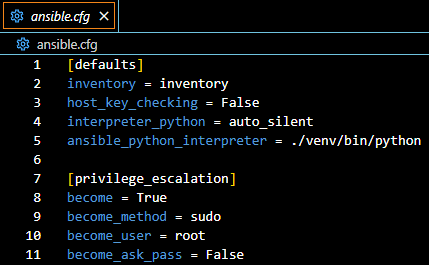
\includegraphics[width=9cm]{images/ansible/0.png}}
      \caption{Fichier ansible.cfg}
      \label{fig:ansible01}
      \end{adjustwidth}
  \end{figure}
  \subsubsection{Fichier main.yaml}
  Cette image illustre le fichier \texttt{main.yaml}, le playbook principal qui orchestre l’ensemble du processus. On y voit les imports des playbooks \texttt{install\_ansible\_dependencies.yaml}, \texttt{setup\_microk8s.yaml}, \texttt{setup\_argocd.yaml}, et \texttt{deploy\_argocd\_application.yaml}, suivis d’une tâche finale affichant des instructions et un résumé des étapes automatisées (installation, configuration, vérification).
  \newpage
  \begin{figure}[h]
    \vspace*{-2cm}
      \begin{adjustwidth}{-3.5cm}{-3.5cm}
      \centering
      \fbox{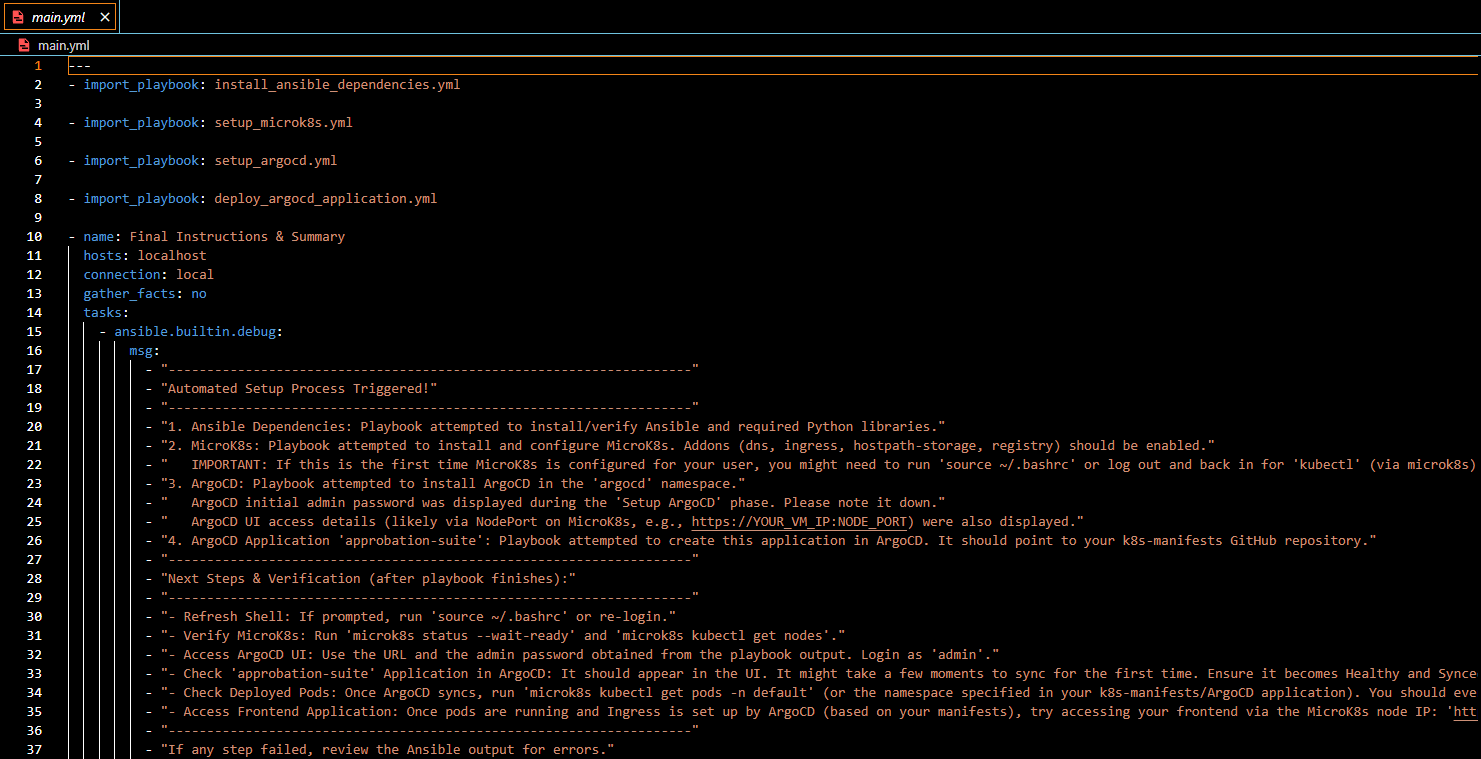
\includegraphics[width=19cm]{images/ansible/2.png}}
      \caption{Fichier main.yaml}
      \label{fig:ansible02}
      \end{adjustwidth}
  \end{figure}
  \subsubsection{Fichier inventory}
Cette image est une capture d’écran du fichier \texttt{inventory}, définissant les hôtes cibles pour Ansible. On y voit la section \texttt{[all]} avec un hôte \texttt{localhost}, une connexion locale, et un interpréteur Python spécifié à \texttt{/opt/ansible\_venv/bin/python3}, configuré pour exécuter les playbooks localement sur la VM.
\begin{figure}[h]
      \begin{adjustwidth}{-3.5cm}{-3.5cm}
      \centering
      \fbox{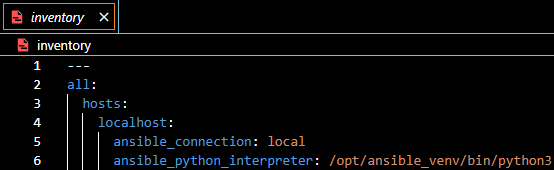
\includegraphics[width=13cm]{images/ansible/3.png}}
      \caption{Fichier inventory}
      \label{fig:ansible03}
      \end{adjustwidth}
  \end{figure}
  \subsubsection{Fichier install\_ansible\_dependencies.yaml}
  Cette image est une capture d’écran du fichier \texttt{install\_ansible\_dependencies.yaml}, un playbook Ansible qui installe les dépendances nécessaires sur la VM Ubuntu. On y voit les tâches pour mettre à jour le cache APT, installer des packages essentiels (comme \texttt{software-properties-common}, \texttt{python3-pip}, \texttt{python3-venv}), ajouter le PPA Ansible, et configurer un environnement virtuel Python.
  \begin{figure}[h]
      \vspace*{-1.5cm}
      \begin{adjustwidth}{-3.5cm}{-3.5cm}
      \centering
      \fbox{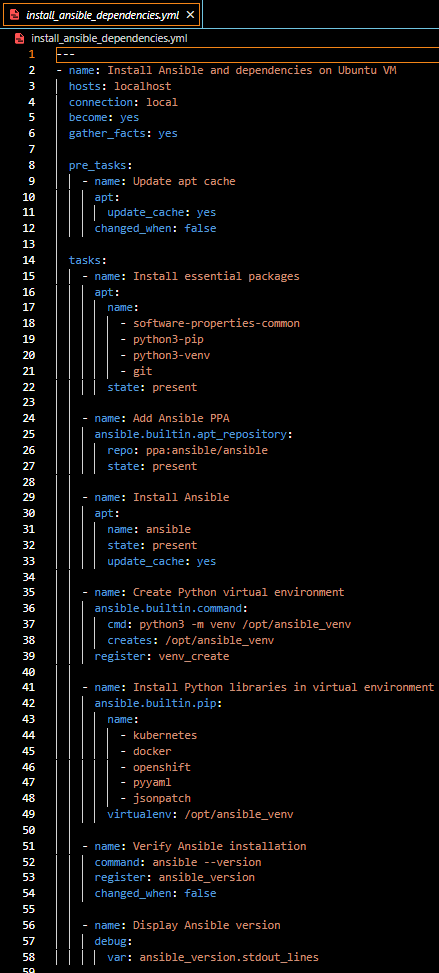
\includegraphics[width=10cm]{images/ansible/4.png}}
      \caption{Fichier install ansible dependencies.yaml}
      \label{fig:ansible04}
      \end{adjustwidth}
  \end{figure}
  \clearpage
\subsubsection{Fichier setup\_microk8s.yaml}
Ce playbook Ansible permet d'automatiser l'installation et la configuration de MicroK8s sur une machine Ubuntu. Il installe MicroK8s via Snap, attend que le service soit prêt, puis active plusieurs modules essentiels tels que \texttt{dns}, \texttt{ingress}, \texttt{hostpath-storage} et \texttt{registry} avec une taille personnalisée. Il est conçu pour être idempotent, c’est-à-dire qu’il peut être relancé sans provoquer d'erreurs si les composants sont déjà installés ou activés.
\begin{figure}[h]
    \begin{adjustwidth}{-3.5cm}{-3.5cm}
    \centering
    \fbox{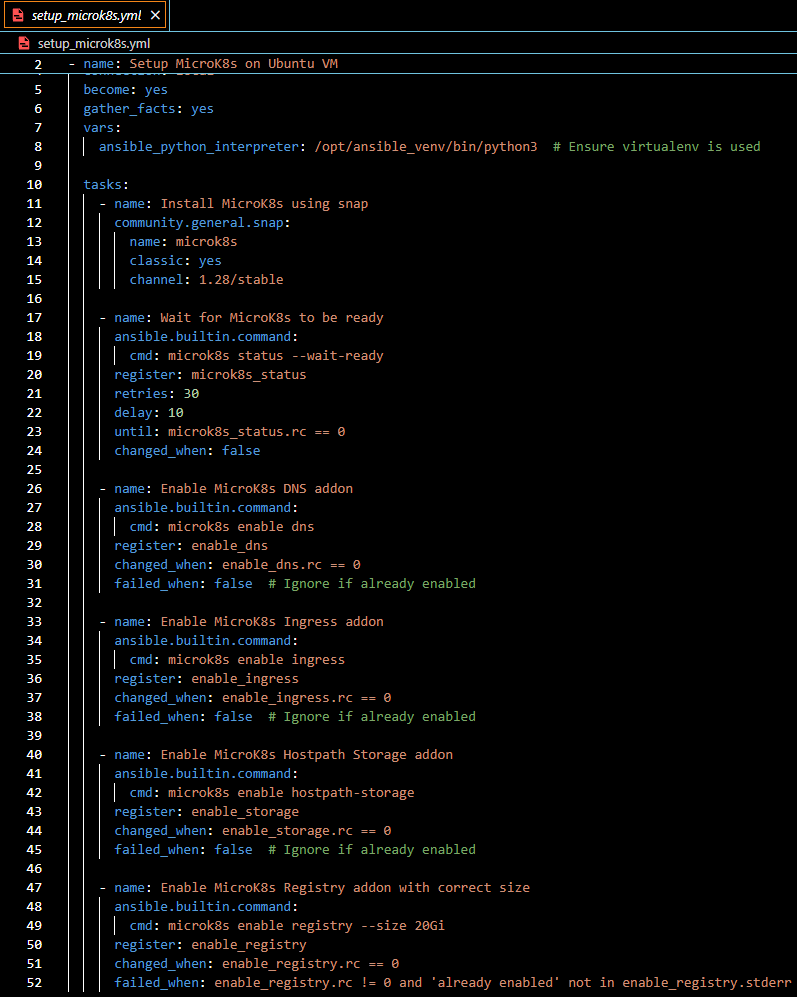
\includegraphics[width=12cm]{images/ansible/5.png}}
    \caption{Fichier setup microk8s.yaml}
    \label{fig:ansible05}
    \end{adjustwidth}
\end{figure}
\newpage
\subsubsection{Fichier setup\_argocd.yaml}
les images \ref{fig:ansible06} et \ref{fig:ansible07} présentent le fichier \texttt{setup\_argocd.yaml}, un playbook Ansible pour installer et configurer ArgoCD. On y voit les tâches créant un namespace ArgoCD, appliquant les manifests d’installation depuis un dépôt GitHub, attendant que le déploiement soit prêt, et récupérant le mot de passe initial de l’administrateur via une commande \texttt{kubectl}.
\begin{figure}[h]
    \begin{adjustwidth}{-3.5cm}{-3.5cm}
    \centering
    \fbox{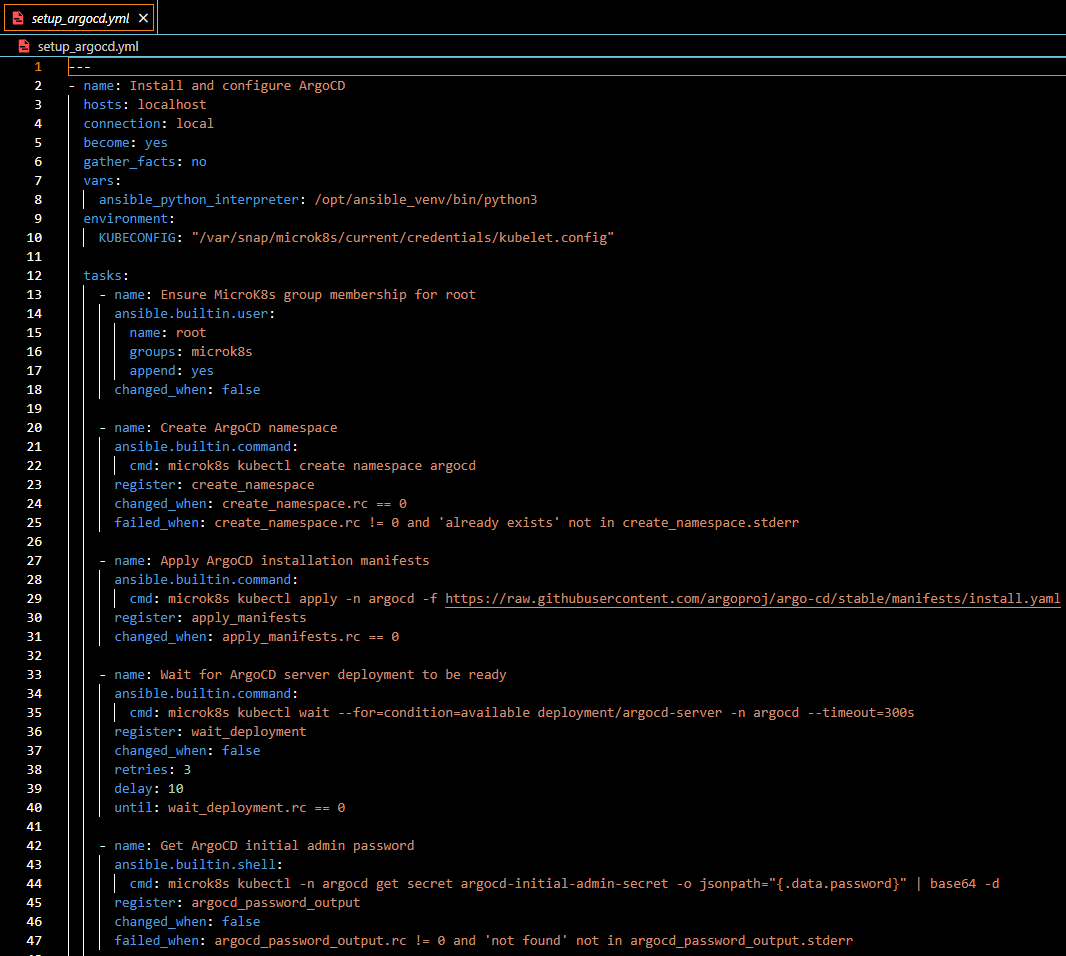
\includegraphics[width=18cm]{images/ansible/6-1.png}}
    \caption{Fichier setup\_argocd.yaml}
    \label{fig:ansible06}
    \end{adjustwidth}
\end{figure}
\newpage
\begin{figure}[h]
    \vspace*{-1cm}
    \begin{adjustwidth}{-3.5cm}{-3.5cm}
    \centering
    \fbox{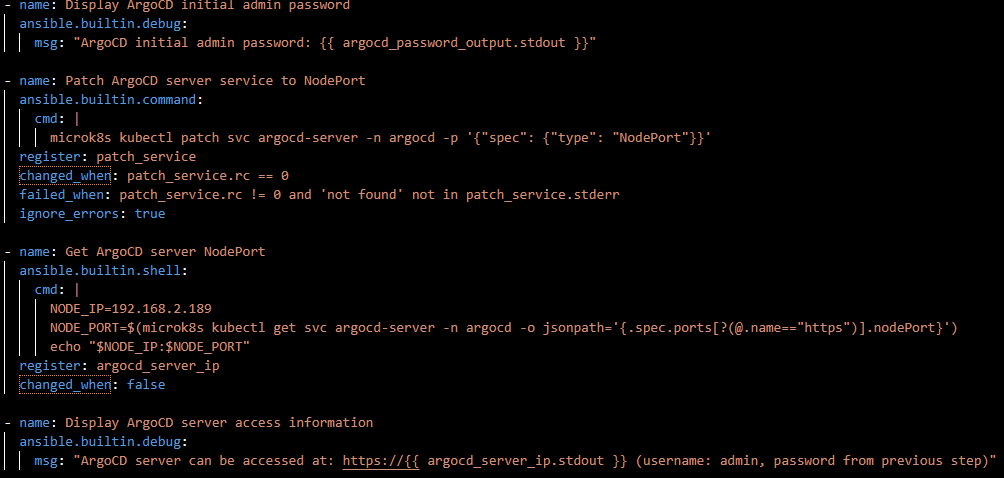
\includegraphics[width=18cm]{images/ansible/6-2.png}}
    \caption{Fichier setup\_argocd.yaml}
    \label{fig:ansible07}
    \end{adjustwidth}
\end{figure}
\subsubsection{Fichier deploy\_argocd\_application.yaml}
Cette image montre le fichier \texttt{deploy\_argocd\_application.yaml}, un playbook Ansible qui déploie une application ArgoCD. On y voit les tâches vérifiant l’existence du fichier manifeste \texttt{argocd-app-of-apps.yaml}, déployant la ressource via \texttt{kubectl}, et vérifiant l’état de l’application avec un délai de 10 secondes, assurant une synchronisation réussie.
\newpage
\begin{figure}[h]
    \begin{adjustwidth}{-3.5cm}{-3.5cm}
    \centering
    \fbox{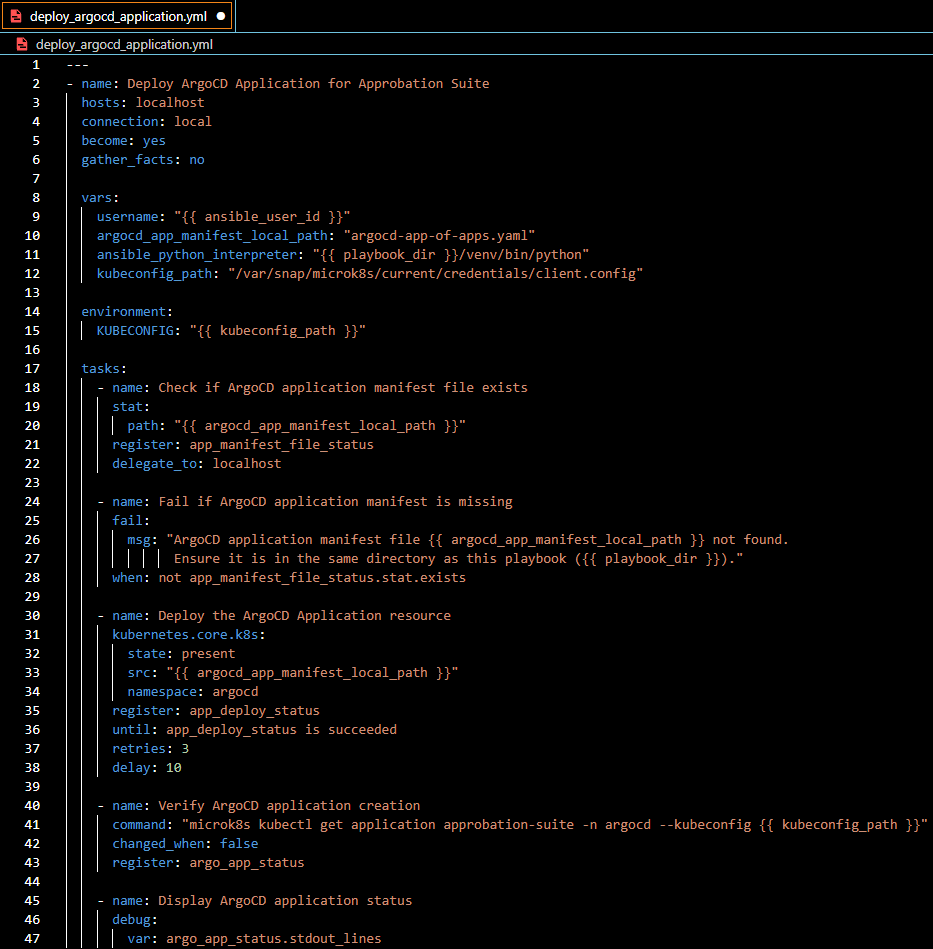
\includegraphics[width=16cm]{images/ansible/7.png}}
    \caption{Fichier deploy\_argocd\_application.yaml}
    \label{fig:ansible08}
    \end{adjustwidth}
\end{figure}

\subsection{Workflows CI}
\subsubsection{Workflow Frontend}
Les images \ref{fig:ansible9} et \ref{fig:ansible10} sont des captures d’écran d’un fichier de configuration GitHub Actions nommé \texttt{.ci.yml}, définissant un pipeline pour le frontend, intitulé \texttt{Frontend Pipeline}. Le workflow est déclenché sur des événements \texttt{push} et \texttt{pull\_request} sur la branche \texttt{main}. Il comprend un job \texttt{build-deploy} exécuté sur un environnement \texttt{ubuntu-latest}, avec plusieurs étapes : checkout du code, configuration de Node.js (version 18), installation des dépendances avec \texttt{npm install}, construction de l’application en mode production avec\\ \texttt{npm run build -- --configuration-production}, configuration de l’environnement Docker avec \texttt{docker/setup-buildx-action} et \texttt{docker/login-action} utilisant des identifiants secrets (\texttt{DOCKERHUB\_USERNAME} et \texttt{DOCKERHUB\_TOKEN}), et enfin la construction et la poussée de l’image Docker avec \texttt{docker buildx build} et \texttt{docker push} vers dockerhub \texttt{approbation-frontend:latest}, en intégrant le hash GitHub (\texttt{github.sha}). Cette image illustre le processus automatisé de construction et de déploiement du frontend.
\begin{figure}[h]
    \begin{adjustwidth}{-3.5cm}{-3.5cm}
    \centering
    \fbox{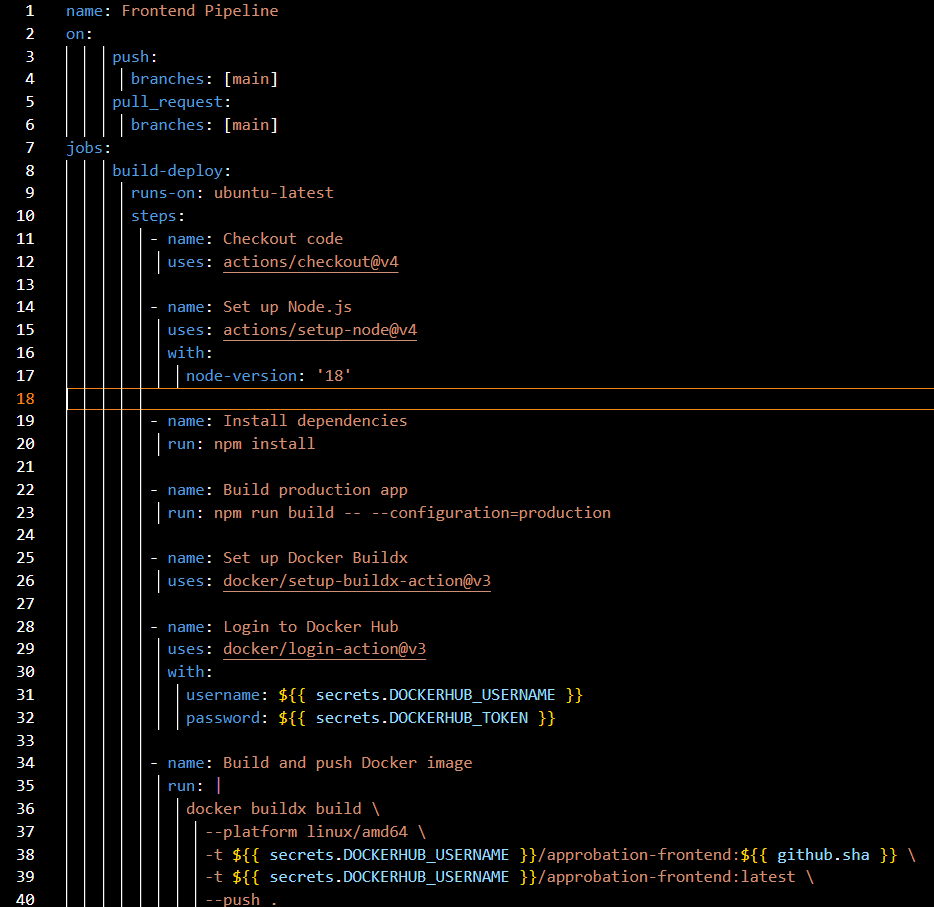
\includegraphics[width=17cm]{images/ansible/9.png}}
    \caption{Fichier Workflow Frontend}
    \label{fig:ansible9}
    \end{adjustwidth}
\end{figure}
\newpage
\begin{figure}[h]
    \begin{adjustwidth}{-3.5cm}{-3.5cm}
    \centering
    \fbox{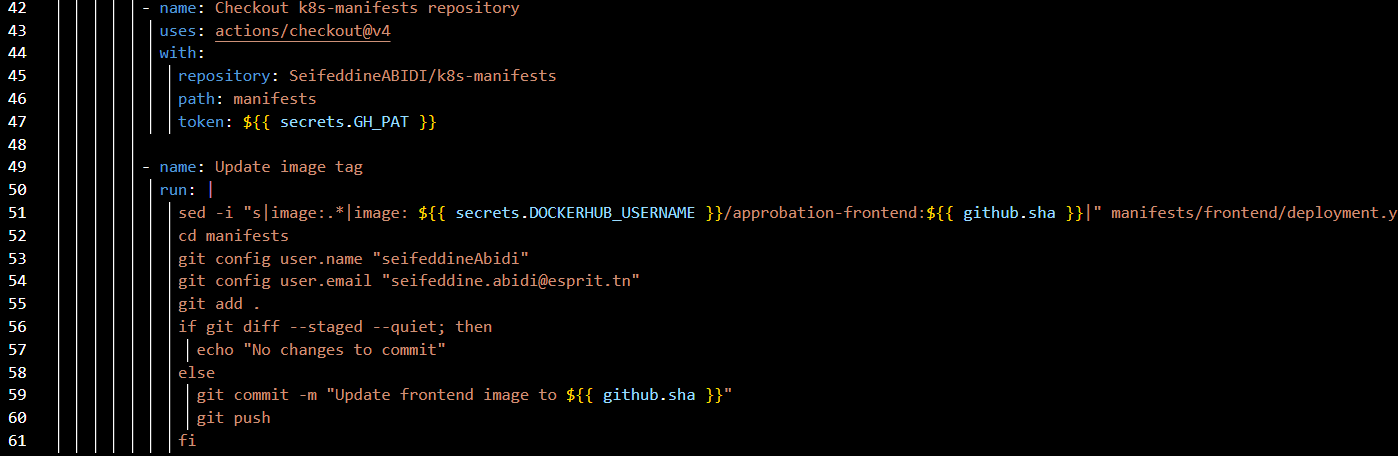
\includegraphics[width=18cm]{images/ansible/10.png}}
    \caption{Fichier Workflow Frontend}
    \label{fig:ansible10}
    \end{adjustwidth}
\end{figure}
\subsubsection{Workflow Backend}
Les images \ref{fig:ansible11} et \ref{fig:ansible12} sont des captures d’écran d’un fichier de configuration GitHub Actions nommé \texttt{.ci.yml}, définissant un pipeline pour le backend, intitulé \texttt{Backend Pipeline}.
Le workflow est déclenché sur des événements \texttt{push} et \texttt{pull\_request} sur la branche \texttt{main}, exécuté sur un runner auto-hébergé (\texttt{self-hosted}).
Les étapes incluent : checkout du code avec une profondeur complète (\texttt{fetch-depth: 0}), configuration de JDK 17 avec \texttt{actions/setup-java}, mise en cache des dépendances Maven pour accélérer les builds, construction avec Maven en sautant les tests (\texttt{mvn clean package -DskipTests}), vérification de la connectivité à SonarQube (via Ingress sur \texttt{192.168.2.189:30000}), et exécution des tests avec JaCoCo pour générer un rapport de couverture.
Cette image met en évidence le processus CI/CD backend, intégrant des analyses statiques et des tests unitaires sur un environnement local.
\newpage
\begin{figure}[h]
    \begin{adjustwidth}{-3.5cm}{-3.5cm}
    \centering
    \fbox{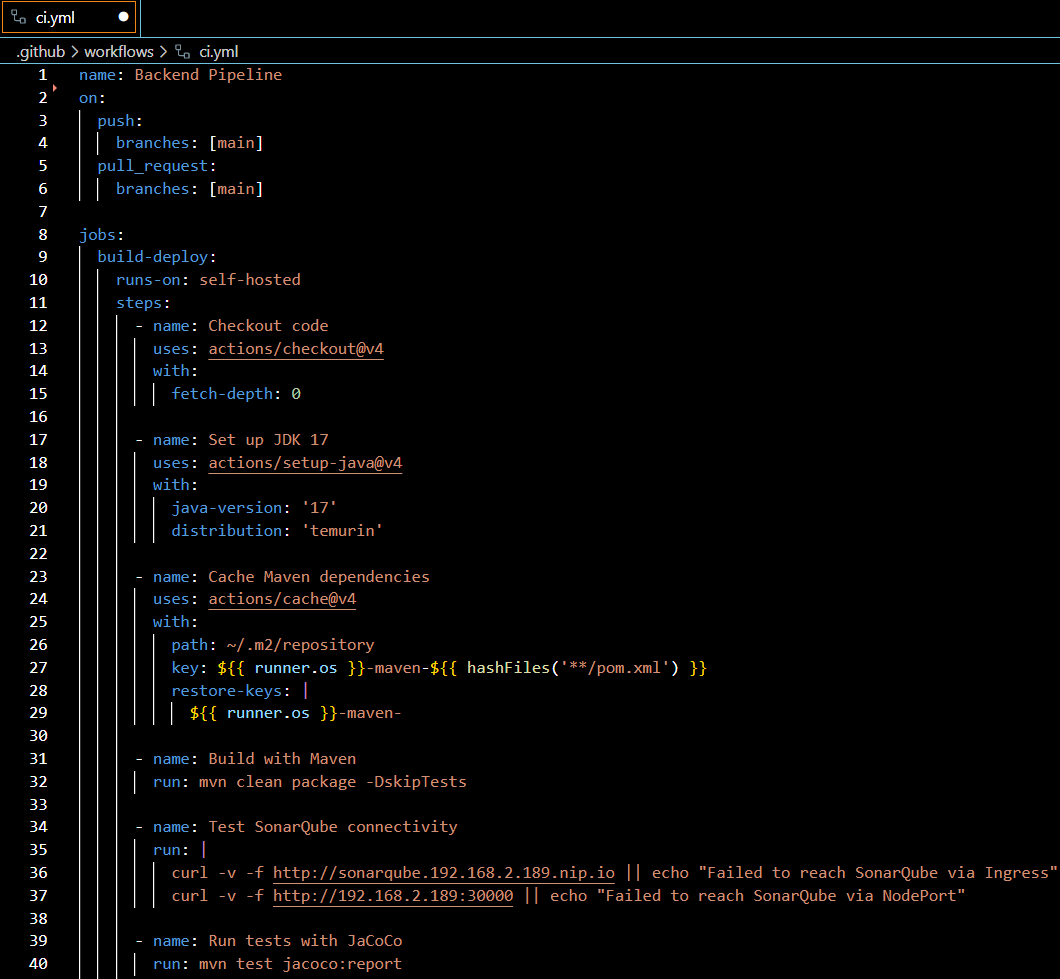
\includegraphics[width=18cm]{images/ansible/11.png}}
    \caption{Fichier Workflow Backend}
    \label{fig:ansible11}
    \end{adjustwidth}
\end{figure}
\newpage
\begin{figure}[h]
    \begin{adjustwidth}{-3.5cm}{-3.5cm}
    \centering
    \fbox{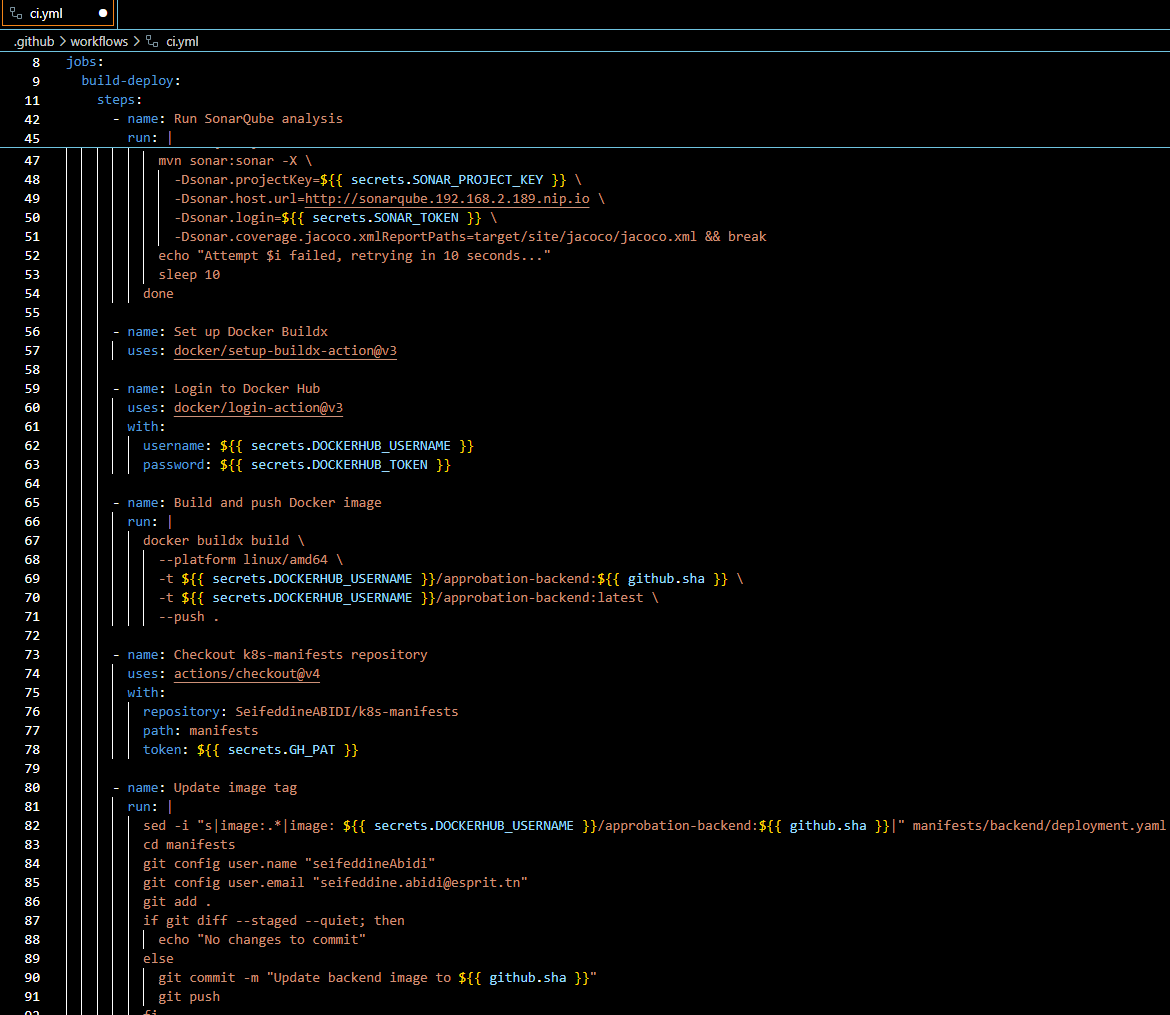
\includegraphics[width=19cm]{images/ansible/12.png}}
    \caption{Fichier Workflow Backend}
    \label{fig:ansible12}
    \end{adjustwidth}
\end{figure}
\subsection{Runner SonarQube}
L'image \ref{fig:ghrun} est une capture d’écran d’un terminal affichant les logs d’un runner GitHub Actions configuré pour exécuter des tâches CI/CD, spécifiquement pour un service backend nommé\\
\texttt{SeifeddineABIDI-Approbation-backend-siga}. Elle montre le démarrage et le fonctionnement du runner sur un environnement Ubuntu VM, avec les détails suivants : le runner est chargé avec le statut \texttt{enabled} et \texttt{preset: enabled},\\
utilisant un fichier de configuration système situé dans:\\ /etc/systemd/system/actions.runner.SeifeddineABIDI-Approbation-backend-siga.service. Les logs indiquent un démarrage réussi à 09:22:35 le 21 mai 2025, avec un PID de 1571 (processus \texttt{runsvc.sh}) et une mémoire utilisée de 171,8 Mo (peak : 173,2 Mo). Le CPU consomme 8,437 secondes, et le runner écoute sur le port 1801. On observe également des tentatives de connexion à GitHub, avec un délai HTTP après 00:00:10 le 21 mai à 09:22:40, suivies d’une reconnexion réussie à 09:51:55, démontrant la résilience du runner face aux interruptions réseau. Cette image illustre la stabilité et la gestion des erreurs du runner auto-hébergé dans un environnement DevOps.
\begin{figure}[h]
    \begin{adjustwidth}{-3.5cm}{-3.5cm}
    \centering
    \fbox{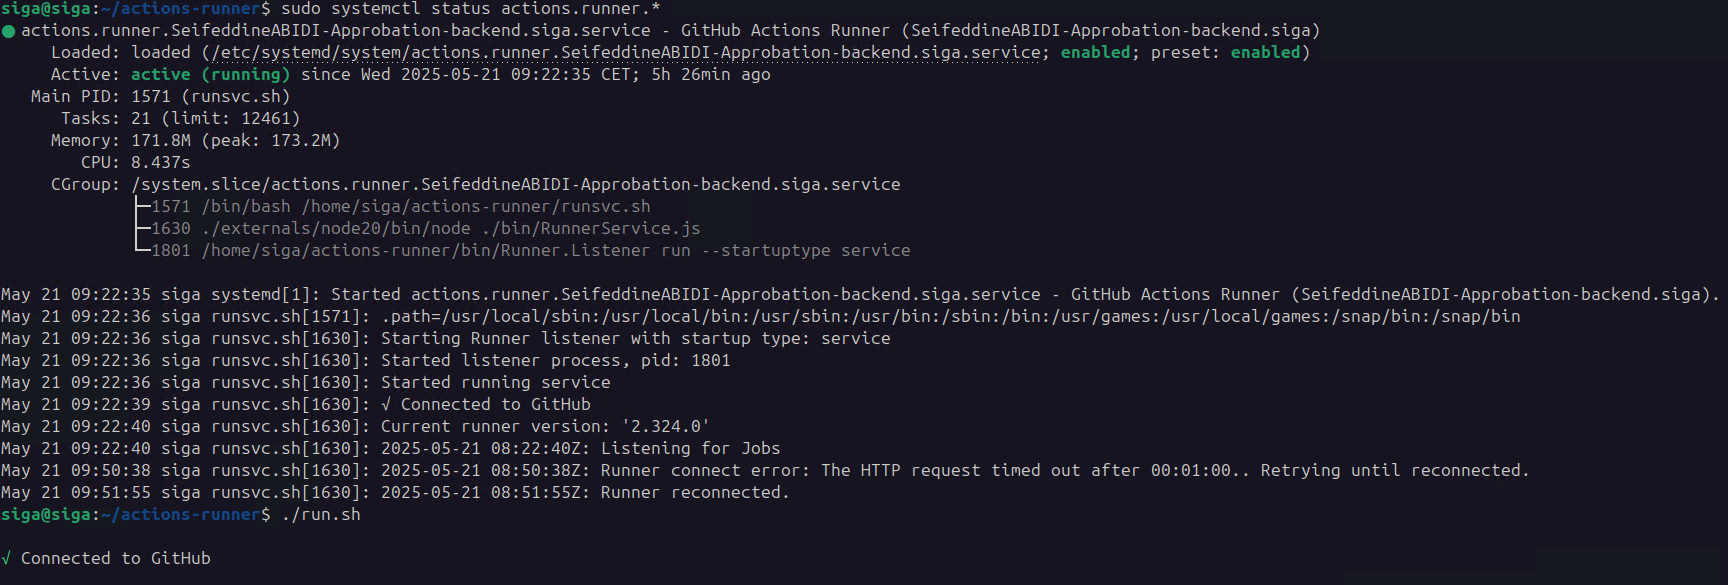
\includegraphics[width=18cm]{images/ansible/8.png}}
    \caption{Capture du Runner GitHub Actions}
    \label{fig:ghrun}
    \end{adjustwidth}
\end{figure}
\subsection{Gestion des Secrets}
L'image \ref{fig:secrkun} est une capture d’écran du fichier \texttt{secrets.yaml}, qui définit plusieurs secrets Kubernetes pour sécuriser les identifiants et mots de passe utilisés dans l’environnement DevOps. Le fichier est structuré en trois ressources de type \texttt{Secret} avec l’API version \texttt{v1}. Le premier secret, nommé \texttt{mysql-credentials}, dans le namespace \texttt{default}, contient des données opaques pour l’utilisateur (\texttt{username}) et le mot de passe (\texttt{password}) encodés en base64 (valeurs masquées comme \texttt{cm9vdA==} et \texttt{c29tZXBhc3N3b3Jk}). Le deuxième secret, nommé \texttt{backend-secrets}, dans le namespace \texttt{default}, inclut un secret JWT (\texttt{jwt-secret}) et un mot de passe par e-mail (\texttt{mail-password}) encodés en base64, ainsi qu’un secret de recaptcha (\texttt{recaptcha-secret}) pour la validation. Le troisième secret, nommé \texttt{postgres-secret}, dans le namespace \texttt{sonarqube}, contient un mot de passe PostgreSQL (\texttt{postgres-password}) encodé en base64 (\texttt{YWRtaW4=}). Cette image illustre la gestion sécurisée des credentials dans Kubernetes, essentielle pour l’authentification et la protection des données dans les pods (MySQL, backend, et SonarQube).
\newpage
\begin{figure}[h]
    \begin{adjustwidth}{-3.5cm}{-3.5cm}
    \centering
    \fbox{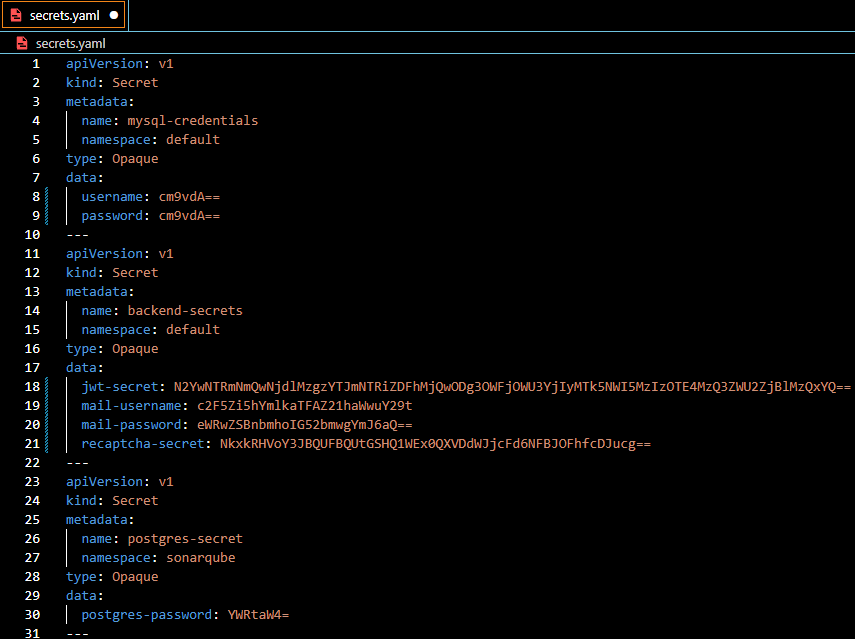
\includegraphics[width=16cm]{images/secrets.png}}
    \caption{Capture du fichier secrets.yaml}
    \label{fig:secrkun}
    \end{adjustwidth}
\end{figure}
\subsection{Exposition des Services}
\subsubsection{Service Frontend}
L'image \ref{fig:fring} est une capture d’écran du fichier \texttt{ingress-frontend.yaml}, qui définit les règles Ingress pour exposer le service frontend dans un cluster MicroK8s. Le fichier utilise l’API \texttt{networking.k8s.io/v1} et spécifie un Ingress nommé \texttt{frontend-ingress} dans le namespace \texttt{default}. Les règles dirigent le trafic HTTP vers le domaine \texttt{frontend.192.168.2.189.nip.io}, acheminant les requêtes vers le service \texttt{frontend-service} sur le port 80. Une annotation \texttt{nginx.ingress.kubernetes.io/rewrite-target: /} est incluse pour réécrire les chemins d’URL, et l’Ingress est configuré pour utiliser un contrôleur Ingress NGINX, assurant un accès externe sécurisé à l’application frontend.
\newpage
\begin{figure}[h]
    \begin{adjustwidth}{-3.5cm}{-3.5cm}
    \centering
    \fbox{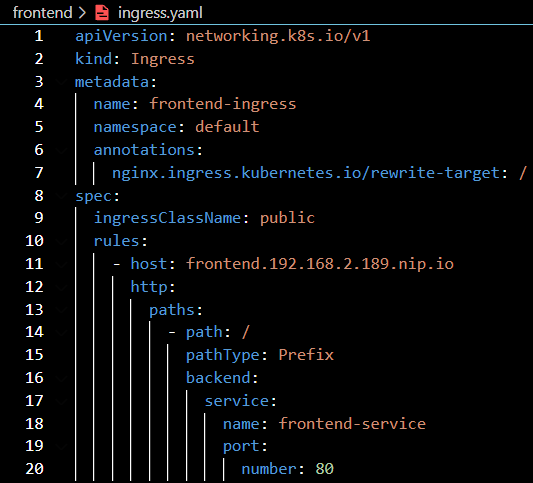
\includegraphics[width=11cm]{images/fring.png}}
    \caption{Fichier ingress-frontend.yaml}
    \label{fig:fring}
    \end{adjustwidth}
\end{figure}
\subsubsection{Service Backend}
L'image \ref{fig:backing} montre le fichier \texttt{ingress-backend.yaml}, qui configure l’exposition du service backend dans le cluster MicroK8s. Le fichier définit un Ingress nommé \texttt{backend-ingress} dans le namespace \texttt{default}, utilisant l’API \texttt{networking.k8s.io/v1}. Les règles associent le domaine \texttt{backend.192.168.2.189.nip.io} au service \texttt{backend-service} sur le port 8080, avec une annotation \texttt{nginx.ingress.kubernetes.io/backend-protocol: HTTP} pour spécifier le protocole. Une configuration supplémentaire pour les limites de taille des requêtes (\texttt{nginx.ingress.kubernetes.io/proxy-body-size: "50m"}) est incluse, permettant la gestion de payloads plus volumineux, comme les appels API du backend.
\newpage
\begin{figure}[h]
    \vspace*{-2cm}
    \begin{adjustwidth}{-3.5cm}{-3.5cm}
    \centering
    \fbox{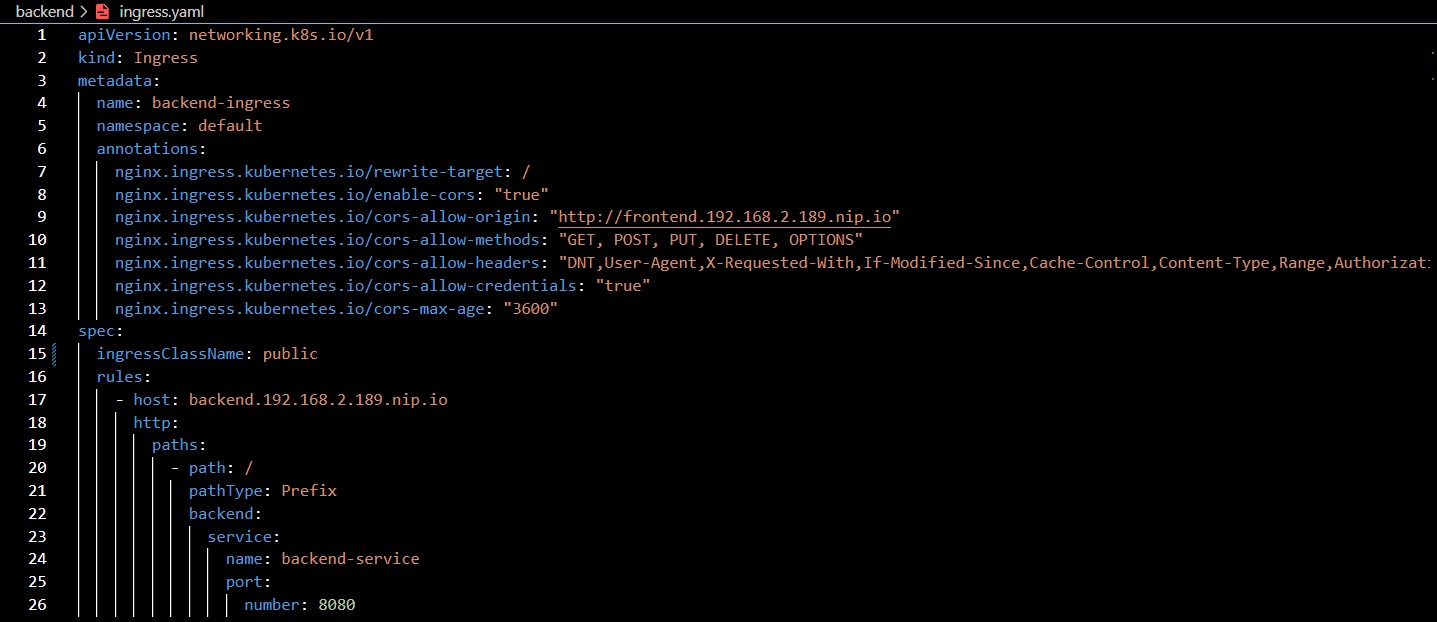
\includegraphics[width=17cm]{images/backing.png}}
    \caption{Fichier ingress-backend.yaml}
    \label{fig:backing}
    \end{adjustwidth}
\end{figure}
\subsubsection{Service SonarQube}
L'image \ref{fig:sonaing} présente le fichier \texttt{ingress-sonarqube.yaml}, qui expose le service SonarQube pour l’analyse de code dans le cluster MicroK8s. L’Ingress, nommé \texttt{sonarqube-ingress}, est défini dans le namespace \texttt{sonarqube} avec l’API \texttt{networking.k8s.io/v1}. Les règles acheminent le trafic du domaine \texttt{sonarqube.192.168.2.189.nip.io} vers le service \texttt{sonarqube-service} sur le port 9000. Une annotation \texttt{nginx.ingress.kubernetes.io/proxy-read-timeout: "300"} est ajoutée pour augmenter le délai d’attente, adapté aux analyses longues de SonarQube, et une annotation \texttt{nginx.ingress.kubernetes.io/ssl-redirect: "false"} désactive la redirection HTTPS pour simplifier l’accès local.
\begin{figure}[h]
    \begin{adjustwidth}{-3.5cm}{-3.5cm}
    \centering
    \fbox{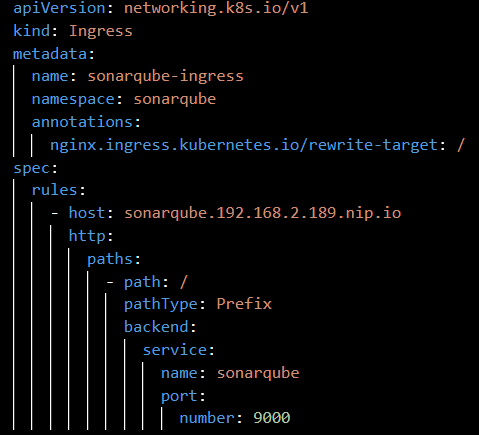
\includegraphics[width=9cm]{images/sonaing.png}}
    \caption{Fichier ingress-sonarqube.yaml}
    \label{fig:sonaing}
    \end{adjustwidth}
\end{figure}
\newpage
\subsection{Surveillance et Rollback}
\subsubsection{Vue générale de l’application}
Cette image montre une capture d’écran de l’interface utilisateur d’ArgoCD, affichant les détails de l’application nommée \texttt{approbation-suite}. L’état de l’application est indiqué comme \texttt{Healthy} et \texttt{Synced to HEAD (083e95d)}, avec une dernière synchronisation réussie le 19 mai 2025 à 06:00 GMT+0100, il y
\begin{figure}[h]
    \begin{adjustwidth}{-3.5cm}{-3.5cm}
    \centering
    \fbox{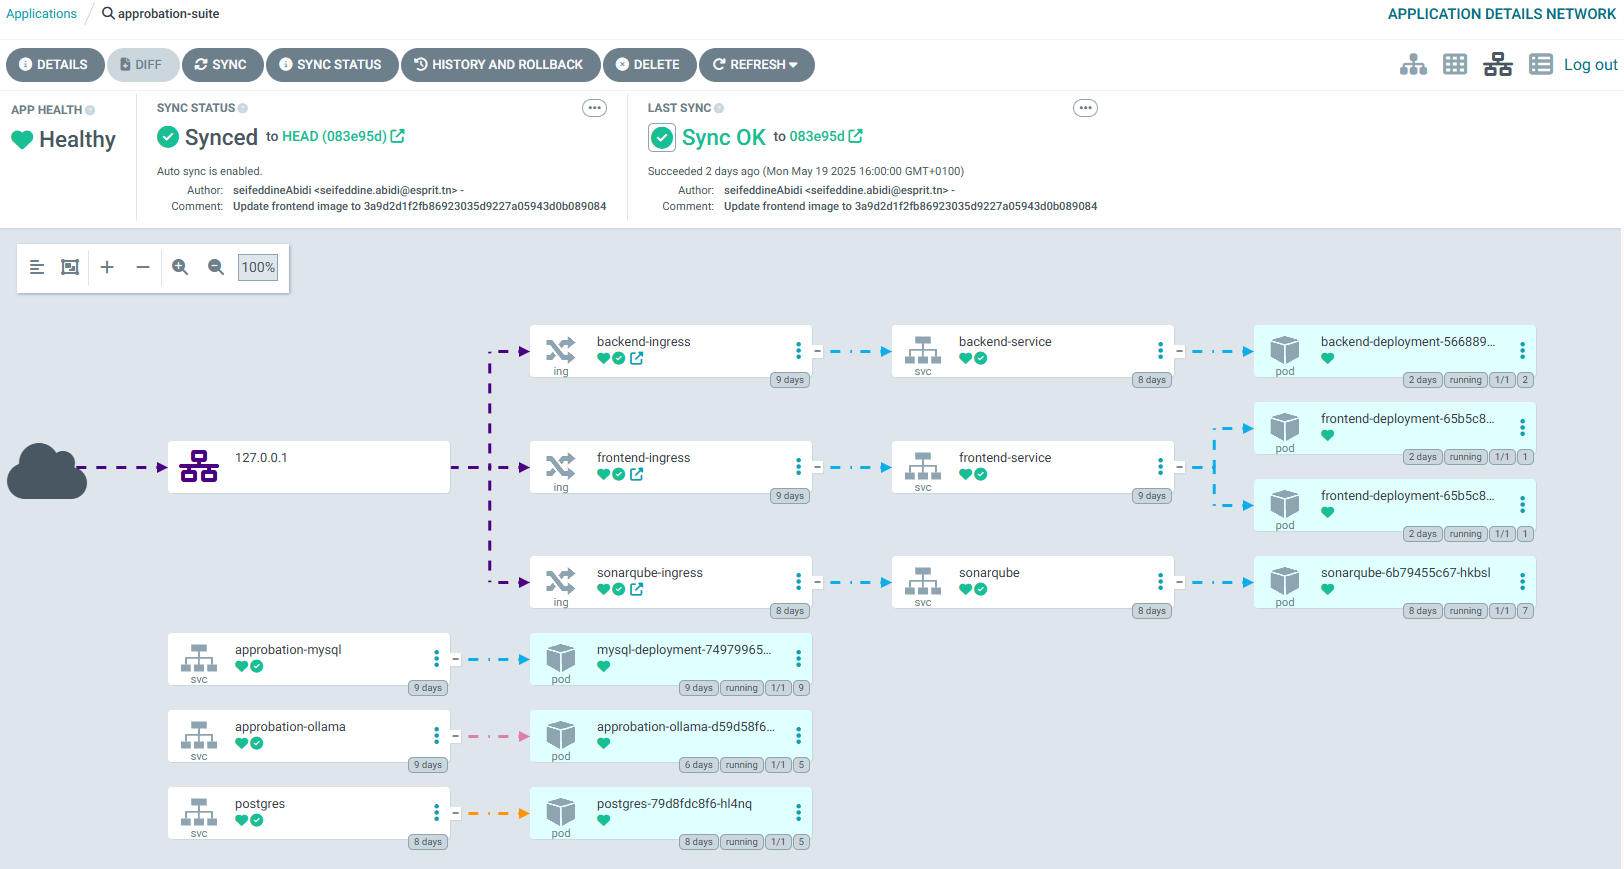
\includegraphics[width=17cm]{images/argo.png}}
    \caption{Interface ArgoCD - Vue générale de l’application "approbation-suite"}
    \label{fig:argo1}
    \end{adjustwidth}
\end{figure}
\subsubsection{Vue des services et secrets}
Cette image illustre une section de l’interface ArgoCD listant les services (SVC) et secrets synchronisés pour l’application \texttt{approbation-suite}. Elle inclut les services \texttt{approbation-mysql}, \texttt{approbation-ollama}, \texttt{backend-service}, \texttt{frontend-service}, \texttt{postgres}, et \texttt{sonarqube}, tous marqués comme synchronisés avec succès depuis 6 à 9 jours. Les secrets associés, tels que \texttt{backend-secrets}, \texttt{mysql-credentials}, et \texttt{postgres-secret}, sont également listés, indiquant une gestion sécurisée des identifiants. Les volumes persistants (PVC) comme \texttt{mysql-pvc}, \texttt{ollama-models}, \texttt{postgres-pvc}, et \texttt{sonarqube-pvc} sont synchronisés depuis 6 à 9 jours, assurant la persistance des données pour les bases de données et les modèles, ce qui souligne la robustesse de l’infrastructure Kubernetes gérée par ArgoCD.
\newpage
\begin{figure}[h]
    \vspace*{-1.5cm}
    \begin{adjustwidth}{-3.5cm}{-3.5cm}
    \centering
    \fbox{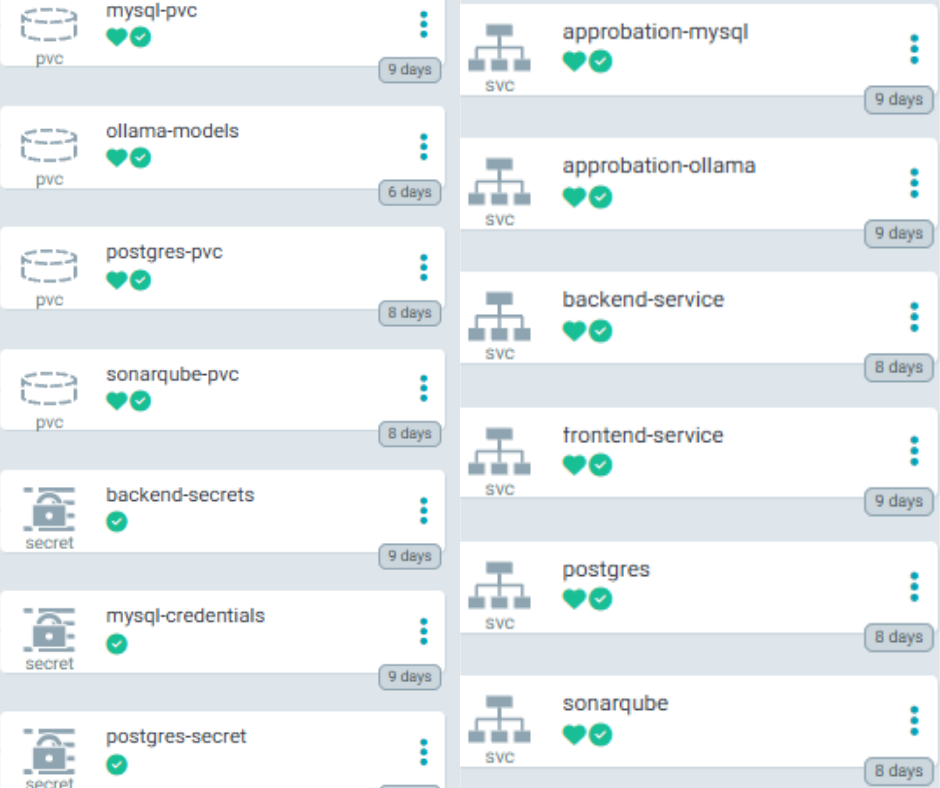
\includegraphics[width=17cm]{images/argo3.png}}
    \caption{Interface ArgoCD - Vue des services et secrets}
    \label{fig:argo2}
    \end{adjustwidth}
\end{figure}
\subsubsection{Vue détaillée des déploiements et pods}
Cette image montre une capture d’écran de l’interface utilisateur d’ArgoCD, affichant les détails de l’application nommée \texttt{approbation-suite}. L’état de l’application est indiqué comme \texttt{Healthy} et \texttt{Synced to HEAD (083e95d)}, avec une dernière synchronisation réussie le 19 mai 2025 à 06:00 GMT+0100, il y a 2 jours. \\L’auteur de la synchronisation automatique est \texttt{seifeddineAbidi-seifeddine.abidi@esprit.tn}, avec un commentaire indiquant une mise à jour de l’image frontend vers un hash GitHub spécifique (\texttt{3a9d21f2b6923035d9227a5943d0b9084}).\\La vue réseau affiche les connexions entre l’adresse IP \texttt{127.0.1} et divers Ingress (\texttt{backend-ingress}, \texttt{frontend-ingress}, \texttt{sonarqube-ingress}), reliant les services (\texttt{backend-service}, \texttt{frontend-service}, \texttt{sonarqube}) à leurs déploiements correspondants (\texttt{backend-deployment}, \texttt{frontend-deployment}, \texttt{sonarqube}) et pods.\\Chaque ressource est marquée comme synchronisée avec succès, avec des durées de fonctionnement allant de 2 à 9 jours, reflétant une infrastructure stable et bien orchestrée.
\begin{figure}[h]
    \begin{adjustwidth}{-3.5cm}{-3.5cm}
    \centering
    \fbox{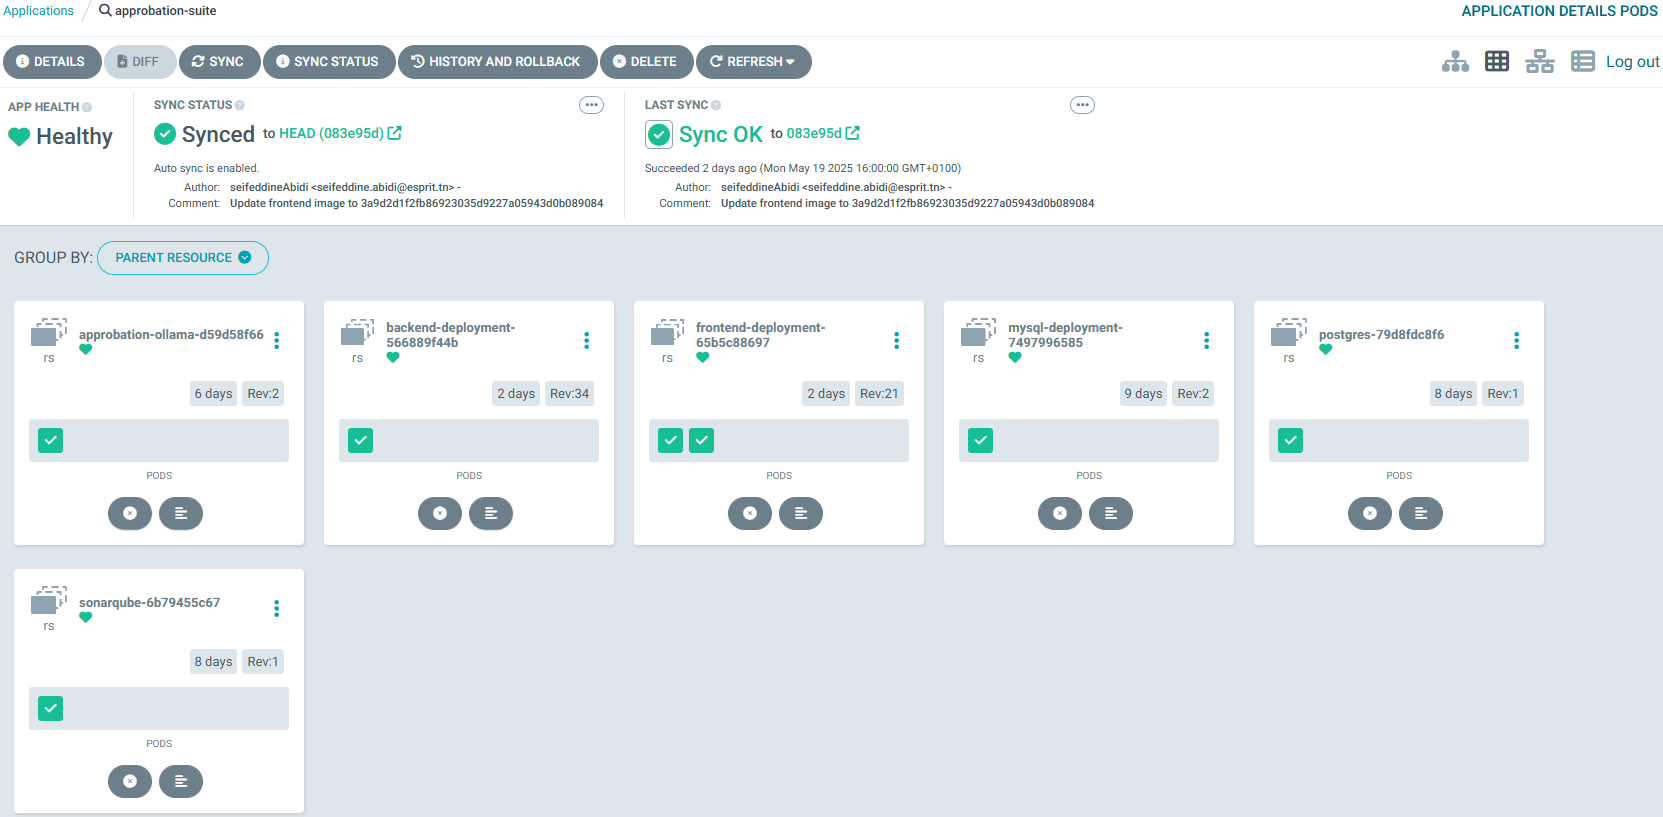
\includegraphics[width=18cm]{images/argo2.png}}
    \caption{Interface ArgoCD - Vue détaillée des déploiements et pods}
    \label{fig:argo3}
    \end{adjustwidth}
\end{figure}
\subsubsection{Tableau de bord de dépoiement}
Le tableau de bord de déploiement Kubernetes présenté dans l'image offre une vue d'ensemble claire de l'état des composants de l'application.\\
Il inclut plusieurs déploiements tels que \texttt{approbation-ollama}, \texttt{backend-deployment}, \texttt{frontend-deployment}, \texttt{mysql-deployment}, \texttt{postgres} et \texttt{sonarqube}, chacun avec des pods en exécution et des durées d'activité variées.\\
Les ressources d'ingress, comme \texttt{backend-ingress}, \texttt{frontend-ingress} et \texttt{sonarqube-ingress}, sont également affichées, garantissant une gestion efficace des accès.\\
Tous les éléments sont marqués comme sains, comme en témoignent les coches vertes, reflétant une infrastructure stable et opérationnelle.
\newpage
\begin{figure}[h]
    \vspace*{-1.5cm}
    \begin{adjustwidth}{-3.5cm}{-3.5cm}
    \centering
    \fbox{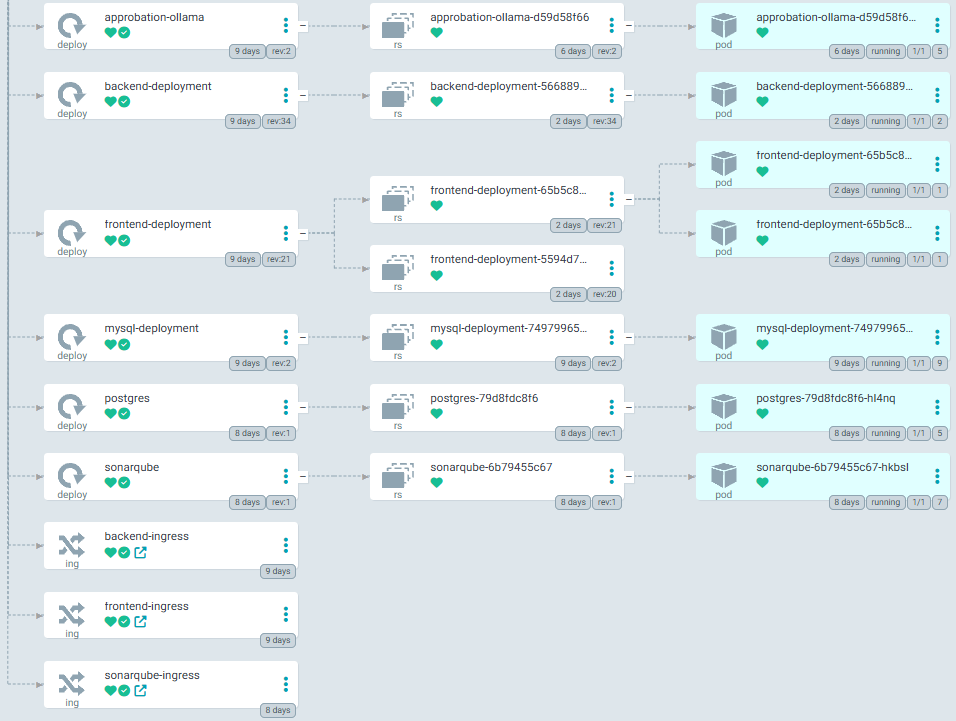
\includegraphics[width=18cm]{images/argo4.png}}
    \caption{Interface ArgoCD - Tableau de bord de dépoiement}
    \label{fig:argo4}
    \end{adjustwidth}
\end{figure}
\subsubsection{Architecture du dépôt des déploiements}
L'architecture du dépôt GitHub illustré dans l'image, nommé \textbf{K8S-MANIFESTS}, contient les fichiers de configuration Kubernetes pour une application multi-composants. L'architecture est organisée en plusieurs dossiers, chacun correspondant à un service spécifique : \texttt{backend}, \texttt{frontend}, \texttt{mysql}, \texttt{ollama}, \texttt{postgres}, \texttt{sonarqube}, ainsi que des fichiers globaux \texttt{kustomization.yaml} et \texttt{secrets.yaml}. Le dossier \texttt{backend} inclut les fichiers \texttt{deployment.yaml}, \texttt{ingress.yaml}, \texttt{kustomization.yaml}, et \texttt{service.yaml}, définissant le déploiement, l'accès réseau, et les services du backend. De manière similaire, le dossier \texttt{frontend} suit la même structure pour l'interface utilisateur. La base de données \texttt{mysql} est configurée via \texttt{deployment.yaml}, \texttt{kustomization.yaml}, \texttt{pvc.yaml} (volume persistant), et \texttt{service.yaml}, utilisée pour stocker les données des applications frontend et backend. Pour \texttt{sonarqube}, qui utilise \texttt{postgres} comme base de données, les fichiers incluent \texttt{deployment.yaml}, \texttt{ingress.yaml}, \texttt{kustomization.yaml}, \texttt{pvc.yaml}, et \texttt{service.yaml}, assurant l'analyse de code avec un stockage persistant via PostgreSQL. Enfin, le dossier \texttt{ollama} gère un composant supplémentaire avec une structure similaire, tandis que les fichiers globaux \texttt{kustomization.yaml} et \texttt{secrets.yaml} centralisent la configuration et les secrets de l'application.
\begin{figure}[h]
    \begin{adjustwidth}{-3.5cm}{-3.5cm}
    \centering
    \fbox{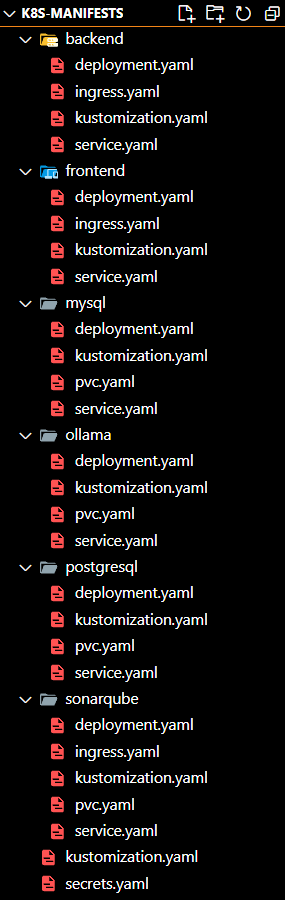
\includegraphics[width=6cm]{images/k8s.png}}
    \caption{Architecture du dépôt des déploiements}
    \label{fig:argo5}
    \end{adjustwidth}
\end{figure}
\clearpage
\section{Conclusion}

Ce chapitre a détaillé le déroulement du Sprint 5, axé sur la mise en place d’un pipeline DevOps et d’une gestion GitOps pour notre plateforme. Grâce à l’intégration de GitHub Actions, nous avons automatisé la construction, les tests et le déploiement des images Docker, en assurant une qualité de code élevée via SonarQube. L’adoption d’ArgoCD et du dépôt \texttt{k8s-manifests} a permis une synchronisation continue et une gestion centralisée des déploiements sur MicroK8s, renforçant la fiabilité grâce à des capacités de surveillance et de rollback. La sécurisation des données sensibles via des secrets Kubernetes et l’exposition des services avec Ingress ont également été des étapes clés pour garantir un accès sécurisé et opérationnel. Ces avancées ont posé des bases solides pour une infrastructure évolutive, maintenable et robuste, tout en optimisant l’efficacité opérationnelle de l’équipe. Ce sprint marque une transition réussie vers des pratiques DevOps et GitOps modernes, prêtes à supporter les évolutions futures du projet.